\documentclass[12pt,a4]{article}

%\usepackage{amsfonts}
%\usepackage[T1]{fontenc}
%\usepackage[utf8]{inputenc}
%\usepackage{amsmath}
%\usepackage{graphicx}

\usepackage[utf8x]{inputenc}
\usepackage[italian]{babel}
\usepackage{graphicx}
\usepackage{amsmath}
\usepackage{amsthm}
\usepackage{amssymb}
\usepackage{listings}
\usepackage{color}
\usepackage[usenames,dvipsnames,table]{xcolor}
\usepackage{fancybox}
%\usepackage[T1]{fontenc}
%\usepackage{tikz}
%\usepackage{tikz-er2}
\usepackage{fancyhdr}
\usepackage{chngpage}
\usepackage{hyperref}

\title{\textbf{Relazione progetto \\ Reti di calcolatori}}
\author{Gianluca Lutero \\  Nicola Mazzara \\ Filippo Soncini}
\date{}

\lstnewenvironment{javacode}
	 { \vspace{4mm}
	 \lstset{
		 frame=tb,
		 language=Java,
		 aboveskip=3mm,
		 belowskip=3mm,
		 showstringspaces=false,
		 columns=flexible,
		 basicstyle={\small\ttfamily},
		 numbers=none,
		 numberstyle=\tiny\color{gray},
		 keywordstyle=\color{blue},
		 commentstyle=\color{gray},
		 stringstyle=\color{black},
		 breaklines=true,
		 breakatwhitespace=true,
		 tabsize=2
	 }
 } {\vspace{4mm}}  


\begin{document}
\maketitle

\newpage
\tableofcontents
\newpage

\section*{Introduzione}
Il progetto realizzato tratta lo sviluppo di un videogioco su piattaforma \textit{Android} che utilizza come interfaccia una mappa, ottenuta da \textit{Google Map}, dove vengono visualizzati i giocatori con i quali si può interagire. In questa relazione verrà prima descritto l'obiettivo dello stesso, il progetto nelle sue componenti di client e server e i protocolli di rete adottati.

\section{Obiettivi}
L'obiettivo che ci siamo prefissati è stato quello di realizzare un server di gioco che mascherasse la sua struttura interna e in grado di servire più client indipendentemente dal tipo di dispositivo. Per questa ragione si è scelto di utilizzare il protocollo http, descritto nella sezione dei protocolli, per la comunicazione client-server e una servlet per realizzare l'interfaccia del server. 

\section{Descrizione del gioco}

\subsection{Client}
Il client di gioco è realizzato su piattaforma Android. Il gioco prevede inizialmente una fase di \textit{login} dopo la quale si accede alla fase di scelta del personaggio e infine alla fase di gioco vera e propria. Di seguito sono descritte le varie funzionalità.

\subsubsection{Login e Registrazione}
L'applicazione prevede una fase di login per accedere al gioco. Una volta effettuato il login il giocatore sceglie il personaggio da usare o ne crea uno nuovo. Se il giocatore non è in possesso di credenziali valide deve effettuare la procedura di registrazione attraverso l'apposita sezione in cui deve fornire una email e una password che lo identificheranno nell'applicazione.

\subsubsection{Creazione del personaggio}
Una volta premuto il bottone di \textit{creazione nuovo personaggio} sarà possibile selezionare uno tra i possibili personaggi disponibili e assegnargli un nome che lo identifica.

\subsubsection{Interfaccia di gioco}
Dopo la scelta del personaggio viene mostrata la mappa alle coordinate del giocatore più gli altri utenti attivi in quel momento. Sulla mappa il giocatore seleziona il personaggio che vuole attaccare.

\subsubsection{Scontro tra i giocatori}
Lo scontro avviene selezionando il personaggio bersaglio e cliccando il bottone apposito. Se il personaggio viene sconfitto questi viene rimosso dalla mappa e al giocatore vengono assegnati 5 punti esperienza.

\subsection{Server}
Il server di gioco è realizzato attraverso una \texttt{Servlet} in Java. Il server riceve le richieste \texttt{Http} del client. Il client invia come parametro il servizio richiesto dal server. Di seguito è descritta la struttura e le funzionalità del server.

\subsubsection{Struttura}
Il server è formato dal \textit{dispatcher}, che fa da interfaccia con i client, dall' \textit{authentication service}, che gestisce la fase di autenticazione e registrazione dell'utente, dal \textit{database service}, che gestisce la comunicazione con il database, e dal \textit{coreapp service}, che gestisce le funzionalità proprie del gioco, e dal database.
\newpage
Nella seguente figura è mostrata la struttura:\\
\\
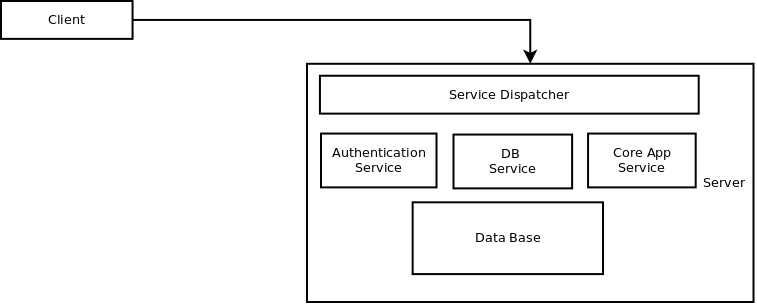
\includegraphics[scale=0.3]{./Schema_Server.png} \\

\subsubsection{Dispatcher}
La parte del server che fa da interfaccia con il client. Il componente riceve le richieste dai client, controlla che siano ben formate e le inoltra ai servizi sottostanti. Il componente attende le risposte dai servizi sottostanti e le restituisce ai client.

\subsubsection{Authentication service}	
La parte del server che fornisce il servizio di autenticazione e registrazione. Se le credenziali sono esatte l'utente viene inserito nella lista degli utenti attivi e viene generato per esso un id di sessione che gli verrà restituito.  

\subsubsection{Database service}
Servizio che fa da interfaccia con il database sottostante.

\subsubsection{Coreapp service}
Implementa tutte le funzionalità lato server dell'applicazione.

\section{Ptotocolli di rete utilizzati}

\subsection{Http}
HTTP (protocollo di trasferimento di un ipertesto) è usato come principale sistema per la trasmissione di informazioni sul web. Un server HTTP generalmente resta in ascolto delle richieste dei client sulla porta 80 usando un protocollo
TCP a livello di trasporto. L'HTTP funziona su un meccanismo richiesta/risposta (client/server): il client esegue una richiesta e il server restituisce la risposta.\\
Il messaggio di richiesta è composto da tre parti:
\begin{itemize}
\item riga di richiesta (request line)
\item sezione header (informazioni aggiuntive)
\item body (corpo del messaggio)
\end{itemize}
Il messaggio di risposta è di tipo testuale ed è composto da tre parti:
\begin{itemize}
\item riga di stato (status-line)
\item sezione header
\item body (contenuto della risposta)
\end{itemize}
Client è server comunicano solo attraverso questo protocollo, in particolare si sfruttano alcuni parametri,descritti in seguito, che generano il linguaggio di comunicazione tra i due. 

\subsubsection{Specifiche dei parametri}
Il client seleziona i servizi nel server attraverso il parametro \texttt{service}. Questo parametro può assumere i seguenti valori:\\
\begin{itemize}
\item  \texttt{signin}: Invoca il servizio di registrazione. Devono essere forniti come parametri l'email e la password.

\item  \texttt{login}: Invoca il servizio di login. Devono essere forniti come parametri l'email e la password, se l'autenticazione ha avuto successo il giocatore viene aggiunto a quelli attivi.

\item \texttt{logout}: Invoca il servizio di logout. Deve essere fornita come parametro l'email del giocatore

\item \texttt{create}: Invoca il servizio di creazione del personaggio. Deve essere fornito l'email del giocatore che lo crea, il nome e la classe del personaggio.

\item \texttt{get\_players}: Invoca il servizio di richiesta dei personaggi di un giocatore. Deve essere fornita l'email del giocatore.

\item \texttt{near player}: Invoca il servizio di richiesta dei giocatori vicini. Deve essere fornito come parametro il nome,la classe, la posizione, l'esperienza e il livello del personaggio che viene inserito tra quelli attivi e poi restituito insieme alla lista dei personaggi.

\item \texttt{logout player}: Invoca il servizio di logout del personaggio. Deve essere fornito il nome del personaggio.

\item \texttt{attack}: Invoca il servizio con cui un personaggio attacca gli altri personaggi. Deve essere fornito il nome dell'attaccante e il nome del difensore.

\end{itemize}

\subsection{Algoritmo crittografico SHA-1}
L'algoritmo sha-1(Secure Hash Algorithm) genera un \textit{message digest} di lunghezza fissa partendo da un messaggio di lunghezza variabile.
\subsubsection{Funzionamento dell'algoritmo}

\textbf{Passo 1} (Imbottitura): Al messaggio originale vengono aggiunti dei bit di "imbottitura" affinché la lunghezza finale del messaggio risulti congruente a 448 modulo 512, così facendo la lunghezza di "messaggio+imbottitura" è pari ad un numero 64bit più piccolo di un multiplo di 512bit.\\
\textbf{Passo 2} (Aggiunta lunghezza): Alla sequenza di bit (messaggio+imbottitura) creata durante il passo 1 viene aggiunto un intero unsigned di 64bit contenente la lunghezza del messaggio originale. Alla fine di questi due primi passi otteniamo una sequenza di bit che è un multiplo di 512.\\
\textbf{Passo 3} (Inizializzazione del buffer MD): Un buffer di 160bit suddiviso in 5 registri da 32bit ciascuno viene creato per la memorizzazione di alcuni passaggi intermedi. I 5 registri verranno convenzionalmente indicati con (A,B,C,D,E) ed inizializzati con i seguenti valori esadecimali:
\begin{itemize}

\item A = 67452301
\item B = EFCDAB89
\item C = 98BADCFE
\item D = 10325476
\item E = C3D2E1F0

\end{itemize}
\textbf{Passo 4} (Elaborazione dei blocchi da 512bit): La sequenza di bit "messaggio+imbottitura+lunghezzaMessaggio" viene divisa in blocchi da 512bit, che identificheremo con Bn con n che va da 0 a L. Il fulcro dell'algoritmo SHA-1 è chiamato compression function ed è formato da 4 cicli di 20 passi cadauno. I cicli hanno una struttura molto simile tra di loro se non per il fatto che utilizzano una differente funzione logica primitiva. Ogni blocco viene preso come parametro di input da tutti e 4 i cicli insieme ad una costante K e i valori dei 5 registri. Alla fine della computazione otterremo dei nuovi valori per A,B,C,D,E che useremo per la computazione del blocco successivo sino ad arrivare al blocco finale F.
Nel progetto l'algoritmo viene utilizzato per criptare le password degli utenti, che varranno salvate nel database in questa forma, usando la libreria Java \texttt{MessageDigest}.\\
Di seguito il codice:
\begin{javacode}
private String cripta(String s) throws NoSuchAlgorithmException{
		  MessageDigest mess = null;
		    mess = MessageDigest.getInstance("SHA-1");
		    mess.reset();
		    try {
				mess.update(s.getBytes("UTF-8"));
			} catch (UnsupportedEncodingException e) {
				e.printStackTrace();
			}
		    
		    byte[] dig = mess.digest();
		    
		    StringBuffer sb = new StringBuffer();
	        for (int i = 0; i < dig.length; i++) {
	          sb.append(Integer.toString((dig[i] & 0xff) + 0x100, 16).substring(1));
	        }
		    
		    System.out.println(sb.toString());
		    
		    return sb.toString();
	}
	
\end{javacode} 

\subsection{Login}
L'utente si autentica nel server invocando il servizio di login e fornendo una email e una password. Il server cerca l'utente nel database e recupera la password criptata associata. A questo punto viene criptata, con algoritmo \textit{sha-1}, la password fornita dall'utente e confrontata con quella del database, se l'operazione ha successo viene generato un id di sessione e restituito all'utente altrimenti viene restituito un messaggio d'errore. \\
Di seguito il codice che effettua il login:
\begin{javacode}
public boolean loginUtente(String email,String password){
		
		String control = null;
		
		Connection connection = null;
		PreparedStatement statement = null;
		ResultSet resultSet = null;
	    
		try{
			connection = databaseConnect();
			statement = connection.prepareStatement("SELECT * FROM utenti WHERE email = ?;");
			statement.setString(1, email);
			resultSet = statement.executeQuery();
		
			resultSet.next();
			
			control = resultSet.getString("pass");			
			
			System.out.println("DB:"+control);
			System.out.println("USER:"+cripta(password));
			
			if(control.equals(cripta(password))){
				return true;
			}
			
		}catch(SQLException s){
			databaseDisconnect(connection, statement, resultSet);
			s.printStackTrace();
		} catch (NoSuchAlgorithmException e) {
		e.printStackTrace();
	    }	
		
		return false;	
	
	}

\end{javacode}

\subsection{Sicurezza delle operazioni}
\subsubsection{Sicurezza del protocollo Http}
Il problema nell'utilizzo del protocollo http sta nel traffico dati in chiaro, inoltre non viene garantita ne l'identità del client ne del server. Per ovviare a questa mancanza può essere usata la versione sicura di http chiamata https che sfrutta un canale cifrato, mediante protocollo SSL, per la comunicazione. Il protocollo https garantisce l'integrità dei dati, l'identità del client e del server.

\subsubsection{Sicurezza del protocollo di login}
Il protocollo di login utilizzato impone che le password vengano salvate e confrontate in versione criptata attraverso l'algoritmo sha-1. Inoltre a login avvenuto l'utente ottiene l'id di sessione per garantire la legalità dell'operazione. 

\subsubsection{Sicurezza del server}
Il server è strutturato in modo tale da avere un'interfaccia con l'esterno, il dispatcher. che ne maschera la struttura interna e controlla che le richieste siano ben formate. Inoltre nel server il database service maschera e gestisce le richieste al database.
\end{document}
